% !TeX root = bash.tex

\section{IV. Regex}
\begin{frame}
\frametitle{What's a regex}
\textbf{Regex}: ``regular expressions''
\newline \newline
It is a string… to match patterns in other strings.
\end{frame}

\begin{frame}[fragile]
\frametitle{What can (and can't) a regex do}
A regex can (attempt to):
\begin{itemize}
    \item Match a cell phone number: \verb|[0-9]{11}|
    \item Match a .com domain: \verb|([A-Za-z0-9-]+\.)+com|
    \item Match \textit{Star Wars} subtitles but not \textit{Star Trek}:
        \verb!m | [tn]|b!\footnote{Credit: \url{https://xkcd.com/1313/}}
        \footnote{The art of regex golf: \url{https://alf.nu/RegexGolf}}
\end{itemize}
It cannnot:
\begin{itemize}
    \item Understand emotion (you want NLP)
    \item Write your essays (you want GPT)
    \item Moderate a Minecraft server (you want a real human)
\end{itemize}
\end{frame}

\begin{frame}
\frametitle{Regex is a mess}
\begin{block}{Quote}
I define UNIX as 30 definitions of regular expressions living under one roof.
\begin{flushright}
    — Donald Knuth\footnote{Digital Typography, ch. 33, p. 649 (1999)}
\end{flushright}
\end{block}

Two dominant standards:
\begin{itemize}
    \item \textbf{ERE} (Extended RegEx, POSIX compliant)
    \item \textbf{PCRE} (Perl Compatible RegEx, used in Perl and Python)
\end{itemize}
Our focus today will be ERE.
\end{frame}

\begin{frame}[fragile]
\frametitle{Regex patterns: \tt{.}}
The dot is the simplest pattern:
\begin{table}
    \centering
    \begin{tabular}{ll}
        \textbf{Pattern}    & \textbf{Matches} \\
        \verb|.|            & any character \\
    \end{tabular}
\end{table}

\begin{example}
    \verb|c.t| matches \tt{cat}, \tt{cut}, and \tt{c t}.
\end{example}

\begin{block}{Note}
    \verb|\.| matches a literal dot. Same goes for \verb|\(| \verb|\[| etc.
\end{block}
\end{frame}

\begin{frame}[fragile]
\frametitle{Regex patterns: \tt{[]}}
Brackets match any of the characters inside, but \verb|^| and \verb|-| are special:
\begin{table}
    \centering
    \begin{tabular}{ll}
        \verb|[aeiou]|      & any vowel \\
        \verb|[^aeiou]|     & anything but a vowel \\
        \verb|[0-9]|        & any digit \\
        \verb|[^A-Za-z]|    & anything but letters \\
    \end{tabular}
\end{table}

\begin{example}
    \verb|[A-C][01][0-9]| matches \tt{A00} up to \tt{C19}.
\end{example}
\end{frame}

\begin{frame}[fragile]
\frametitle{Regex patterns: character classes}
\begin{table}
    \centering
    \begin{tabular}{ll}
        \verb|\w|           & \verb|[A-Za-z0-9_]| \\
        \verb|\W|           & anything \verb|\w| does not match \\
        \verb|\s|           & whitespace (space, tab, linebreak, etc) \\
        \verb|\S|           & anything but whitespace \\
    \end{tabular}
\end{table}

\begin{block}{Note}
    Character classes in brackets like \verb|[\w\s]| won't work.
\end{block}
\end{frame}

\begin{frame}[fragile]
\frametitle{Regex patterns: \tt{| ()}}
Vertical bars separate patterns, and matches one of them.
Parentheses can be used to group patterns.
\begin{table}
    \centering
    \begin{tabular}{ll}
        \verb![bc]at|[dh]og!        & bat, cat, dog, or hog \\
        \verb!(ls|cd|rm -r) dir!    & \tt{ls dir}, \tt{cd dir}, or \tt{rm -r dir} \\
    \end{tabular}
\end{table}
\end{frame}

\begin{frame}[fragile]
\frametitle{Regex patterns: repeat}
A repeated pattern can be matched:
\begin{table}
    \centering
    \begin{tabular}{ll}
        \verb|A?|           & zero or one A \\
        \verb|A+|           & one or more A's \\  % Positive closure
        \verb|A*|           & zero or more A's \\ % Kleene closure
        \verb|A{6}|         & 6 A's \\
        \verb|A{4,6}|       & 4--6 A's \\
        \verb|A{4,}|        & more than 4 A's \\
    \end{tabular}
\end{table}

\begin{example}
    \verb|[0-9]{1,3}(,[0-9]{3})*| matches \tt{13} and \tt{420,691,337}.
\end{example}
\end{frame}

\begin{frame}[fragile]
\frametitle{Regex patterns: location}
These do not match literal characters. Instead, they specify the location of
the character before/after it.
\begin{table}
    \centering
    \begin{tabular}{ll}
        \verb|^|            & beginning of string \\
        \verb|$|            & end of string \footnote{Beginning or end of line sometimes} \\
        \verb|\b|           & word boundary \\
        \verb|\B|           & not word boundary \\
    \end{tabular}
\end{table}

\begin{example}
    \begin{itemize}
        \item \verb|^$| matches an empty string only
        \item \verb|\bwork\B| matches \tt{bash workshop} and \tt{worker},
            but not \tt{homework}
    \end{itemize}
\end{example}
\end{frame}

\begin{frame}[fragile]
\frametitle{Quiz: Does it match?}
What strings does this regex match? \newline

\Large \verb!^cat|cat$! \normalsize

\begin{itemize}
    \item \verb|cat|                      % yes
    \item \verb|^cat$|                    % no
    \item \verb|cats|                     % yes
    \item \verb|cat /etc/fstab|           % yes
    \item \verb|I have a cat.|            % no
    \item \verb|Cats are the best.|       % no
    \item \verb|Concatenate these files|  % no
\end{itemize}
\end{frame}

\begin{frame}[fragile]
\frametitle{Quiz: Does it match?}
What matches \tt{+86 021} but not \tt{+86021}?
\begin{itemize}
    \item \verb|\+86\s+[0-9]{3}| % this one
    \item \verb|\+86\s*[0-9]{3}|
\end{itemize}

What does \Large \verb|[um]jicanvas.com| \normalsize match?
\begin{itemize}
    \item \tt{umjicanvas.com}
    \item \tt{jicanvas.com} % neither
\end{itemize}

\begin{block}{Challenge}
    How to fix this regex? % (um)?jicanvas\.com
\end{block}
\end{frame}

\begin{frame}[fragile]
\frametitle{But how to use a regex, anyway?}
Try this in \tt{04-regex/}:
\begin{lstlisting}[language=bash]
$ grep -E '.+\..+@sjtu.edu.cn' faculty
\end{lstlisting}
\pause
\begin{block}{Observation}
    The regex matches all email addresses in the file \tt{faculty}
    that look like ``firstname.lastname@sjtu.edu.cn''.
    \newline \newline
    \tt{-E} stands for Extended regex.
\end{block}
\end{frame}

\begin{frame}[fragile]
\frametitle{One more example}
Try this in \tt{04-regex/}:
\begin{lstlisting}[language=bash]
$ grep -oE '^[^@]{,8}' faculty
\end{lstlisting}
\pause
\begin{block}{Observation}
    ``@sjtu.edu.cn'' are all gone, and each line is at most 8 characters long.
\end{block}
\begin{block}{Explanation}
    \begin{tabular}{ll}
        \verb|^|    & From beginning of each line \\
        \verb|[^@]| & Keep any character except @ \\
        \verb|{,8}| & Until we reach length 8
    \end{tabular}
\end{block}
\end{frame}

\begin{frame}[fragile]
\frametitle{Your turn}
Extract all course codes from \tt{04-regex/courses}. \newline

\begin{example}
    \begin{tabular}{lcl}
        VG100 Introduction to Engineering & & VG100 \\
        VM020 Machineshop Training & $\Longrightarrow$ & VM020 \\
        VP140 Physics I & & VP140
    \end{tabular}
\end{example}
\pause
\begin{block}{Solution (naïve version)}
\begin{lstlisting}[language=bash]
$ grep -oE 'V[A-Z][0-9]+' courses
\end{lstlisting}
\end{block}
\end{frame}

\begin{frame}[fragile]
\frametitle{Find and replace with \tt{sed}}
\tt{sed} is a powerful tool for transforming text.
We will be using one very specific syntax for substitution:\footnote{
    When the pattern/replacement contains slashes, you can use things like
    \tt{!} and \tt{,} as delimiters.
}
\begin{lstlisting}[language=bash]
$ COMMAND | sed -E 's/FIND/REPLACE/FLAGS'
$ sed -E 's/FIND/REPLACE/FLAGS' FILE
\end{lstlisting}
\tt{-E} again stands for Extended regex, and flags are optional.
This command redacts all the IPv4 addresses in the file \tt{ipv4}:
\begin{lstlisting}[language=bash]
$ sed -E 's/([0-9]{1,3}\.){3}[0-9]{1,3}/redacted/g' \
    ipv4
\end{lstlisting}
\begin{block}{Observe}
    What will happen without the \tt{g} at the end?
\end{block}
\end{frame}

\begin{frame}[fragile]
\frametitle{Capturing groups}
A \textbf{capturing group}, or simply \textbf{group}, is a pattern inside
parentheses that mark a region of text you want to keep in the replaced text.
\newline \newline
It can be accessed with a respective \textbf{backreference} which looks like
\verb|\1|, \verb|\2|, up to \verb|\9|.

When nested, the position of \verb|(| determines order, so the outside group is
\verb|\1| and the inside is \verb|\2|.
\end{frame}

\begin{frame}[fragile]
\frametitle{Capturing groups with \tt{sed}}
What if you only want to redact the subnet (i.e. last part) of the IP addresses?
\begin{lstlisting}[language=bash]
$ sed -E 's/(([0-9]{1,3}\.){3})[0-9]{1,3}/\1xxx/g' \
    ipv4
\end{lstlisting}
\begin{block}{Observation}
    IP addresses like \tt{192.168.1.1} become \tt{192.168.1.xxx}
\end{block}
\end{frame}

\begin{frame}[fragile]
\frametitle{Your turn}
From \tt{04-regex/courses}, select 100- and 200-level math courses and convert
legacy ``VV'' course codes into modern ``MATH'' codes.
Do not print other courses.
\begin{example}
    \begin{tabular}{lcl}
        VV156 & & MATH1560J \\
        VV214 & $\Longrightarrow$ & MATH2140J \\
        VV417 & & \textit{not printed}
    \end{tabular}
\end{example}
\pause
\begin{block}{Solution}
\begin{lstlisting}[language=bash]
$ grep -E 'VV[1-2]' courses | \
    sed -E 's/VV([0-9]{3})/MATH\10J/'
\end{lstlisting}
\end{block}
\end{frame}

\begin{frame}
\frametitle{When (and when not) to use regex?}
\begin{figure}[h]
    \centering
    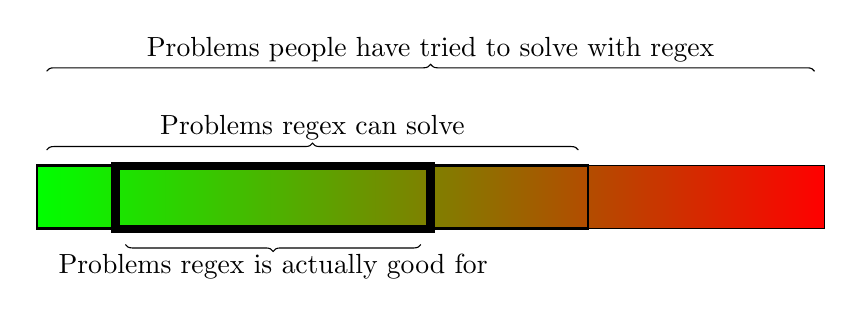
\begin{tikzpicture}
        \node (can-low)     at ( 0,  1)   {};
        \node (can-high)    at ( 7,  1)   {};
        \node (have-low)    at ( 0,  2)   {};
        \node (have-high)   at (10,  2)   {};
        \node (should-low)  at ( 1, -0.2) {};
        \node (should-high) at ( 5, -0.2) {};
        \draw[left color=green, right color=red] (0, 0) rectangle (10, 0.8);
        \draw[line width=1pt] (0, 0) rectangle (7, 0.8);
        \draw[line width=3pt] (1, 0) rectangle (5, 0.8);
        \draw[decorate, decoration=brace] (can-low) -- (can-high)
            node[text centered, midway, above] {Problems regex can solve};
        \draw[decorate, decoration=brace] (have-low) -- (have-high)
            node[text centered, midway, above] {Problems people have tried to solve with regex};
        \draw[decorate, decoration={brace, mirror}] (should-low) -- (should-high)
            node[text centered, midway, below] {Problems regex is actually good for};
    \end{tikzpicture}
\end{figure}
Regex is \textbf{not} the solution to everything. Stop before it is too late.
\end{frame}

